\documentclass[12pt]{article}
\usepackage{fontspec}
\setmainfont{Arial}
\usepackage{setspace}
\singlespacing

\usepackage{graphicx}
\usepackage{caption}
\usepackage[T1]{fontenc}
\usepackage[utf8]{inputenc}
\usepackage{lmodern}
\usepackage{geometry}
\geometry{
	a4paper,
	left=20mm,
	right=20mm,
	top=25mm,
	bottom=25mm,
}

\usepackage{pgfgantt}
\usepackage{eurosym}
\usepackage{pdfpages}


\usepackage{subcaption}

\usepackage[unicode=true,pdfusetitle,bookmarks=true,bookmarksnumbered=false,bookmarksopen=false,
breaklinks=false,pdfborder={0 0 0},backref=false,colorlinks=true,urlcolor=blue]{hyperref}

\usepackage{multibib}
\newcites{article,conf,confnoproc}{{Articles dans des revues internationales à comité de lecture
	},{Communications dans des congrès internationaux à comité de lecture et actes
		publiés},{Communications dans des congrès internationaux sans comité de lecture}}

\graphicspath{{images/}}

\author{Andrea Brugnoli \\ 
	\hspace{2.8pt} Docteur ISAE-Supaéro 2020\\
	Ingénieur ISAE-Supaéro 2017}
\title{Project MORPHEUS \\
	\vspace{.3cm}
	\Large{Model Order Reduction for multi-PHysical and Energy-Unified Systems}  }

\date{}

\begin{document}
	
	\maketitle
	
	\large{Application for the Jean-Jacques and Felicia Lopez-Loreta Foundation Award for Academic Excellence.}
	
	
	\begin{figure}[h]
		\centering
		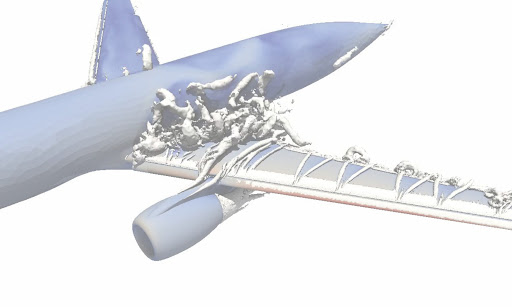
\includegraphics[width=.95\textwidth]{3Dplane.jpg}
		\captionsetup{labelformat=empty}
		\caption{Source: \href{http://www.fenics-hpc.org/}{FEniCS-HPC website}}
	\end{figure}
	
	
	
	
	
	\thispagestyle{empty}
	
	\newpage
	
	\section{Project summary}
	
	The goal of the MORPHEUS project is to implement numerical methods 	to accelerate the simulation of fluid-structure interaction (FSI) problems, compared to the computational time required for a high-fidelity simulation. It will thus be possible to integrate more economical models, which can replace very expensive simulations, and thus facilitate optimized component design and decision making. Unlike many methods proposed in the literature, the imperative is fidelity to the physical structure of the problem.  This structure is most often ignored by reduction algorithms, which treat simulations as black boxes. Physically faithful reduced models are much more accurate, and their use can radically improve the techniques normally used for model reduction and optimization. To achieve its ambition, this project aims at using recent mathematical formalisms for multiphysics modeling and model digitization. Tools capable of accurately predicting the behavior of complex systems are of fundamental importance to help us face future technological and societal challenges. The fact that this year's Nobel Prize in Physics was awarded to three researchers working on this topic\footnote{\url{https://www.nobelprize.org/prizes/physics/2021/summary/}} confirms the importance and topicality of this subject.

	
	\section{Scientific project development}
	
	\subsection{Multiphysics problems}
	Computational engineering is a recent, multidisciplinary, and rapidly expanding science. Its goal is to implement mathematical and numerical models to predict the behavior of complex systems. This allows to avoid the use of experimental tests which are very costly for systems in the design phase and to detect faults during the life cycle of the components. This field is rapidly expanding because today we have more powerful computers and especially because, thanks to the development of open source codes, the software is much more accessible, robust and easy to use. However, multiphysics problems, which are central in industrial applications, are extremely complicated to deal with. This is due on the one hand to the difficulty associated with the treatment of the different physics and on the other hand to the size of the systems obtained, which require several days, even several weeks, to be solved using a supercomputer. These problems pose barriers for the use of numerical models in industry. 
	
	
	
	\subsection{Scientific tools of the MORPHEUS project}
	
	\begin{figure}[tb]
		\centering
		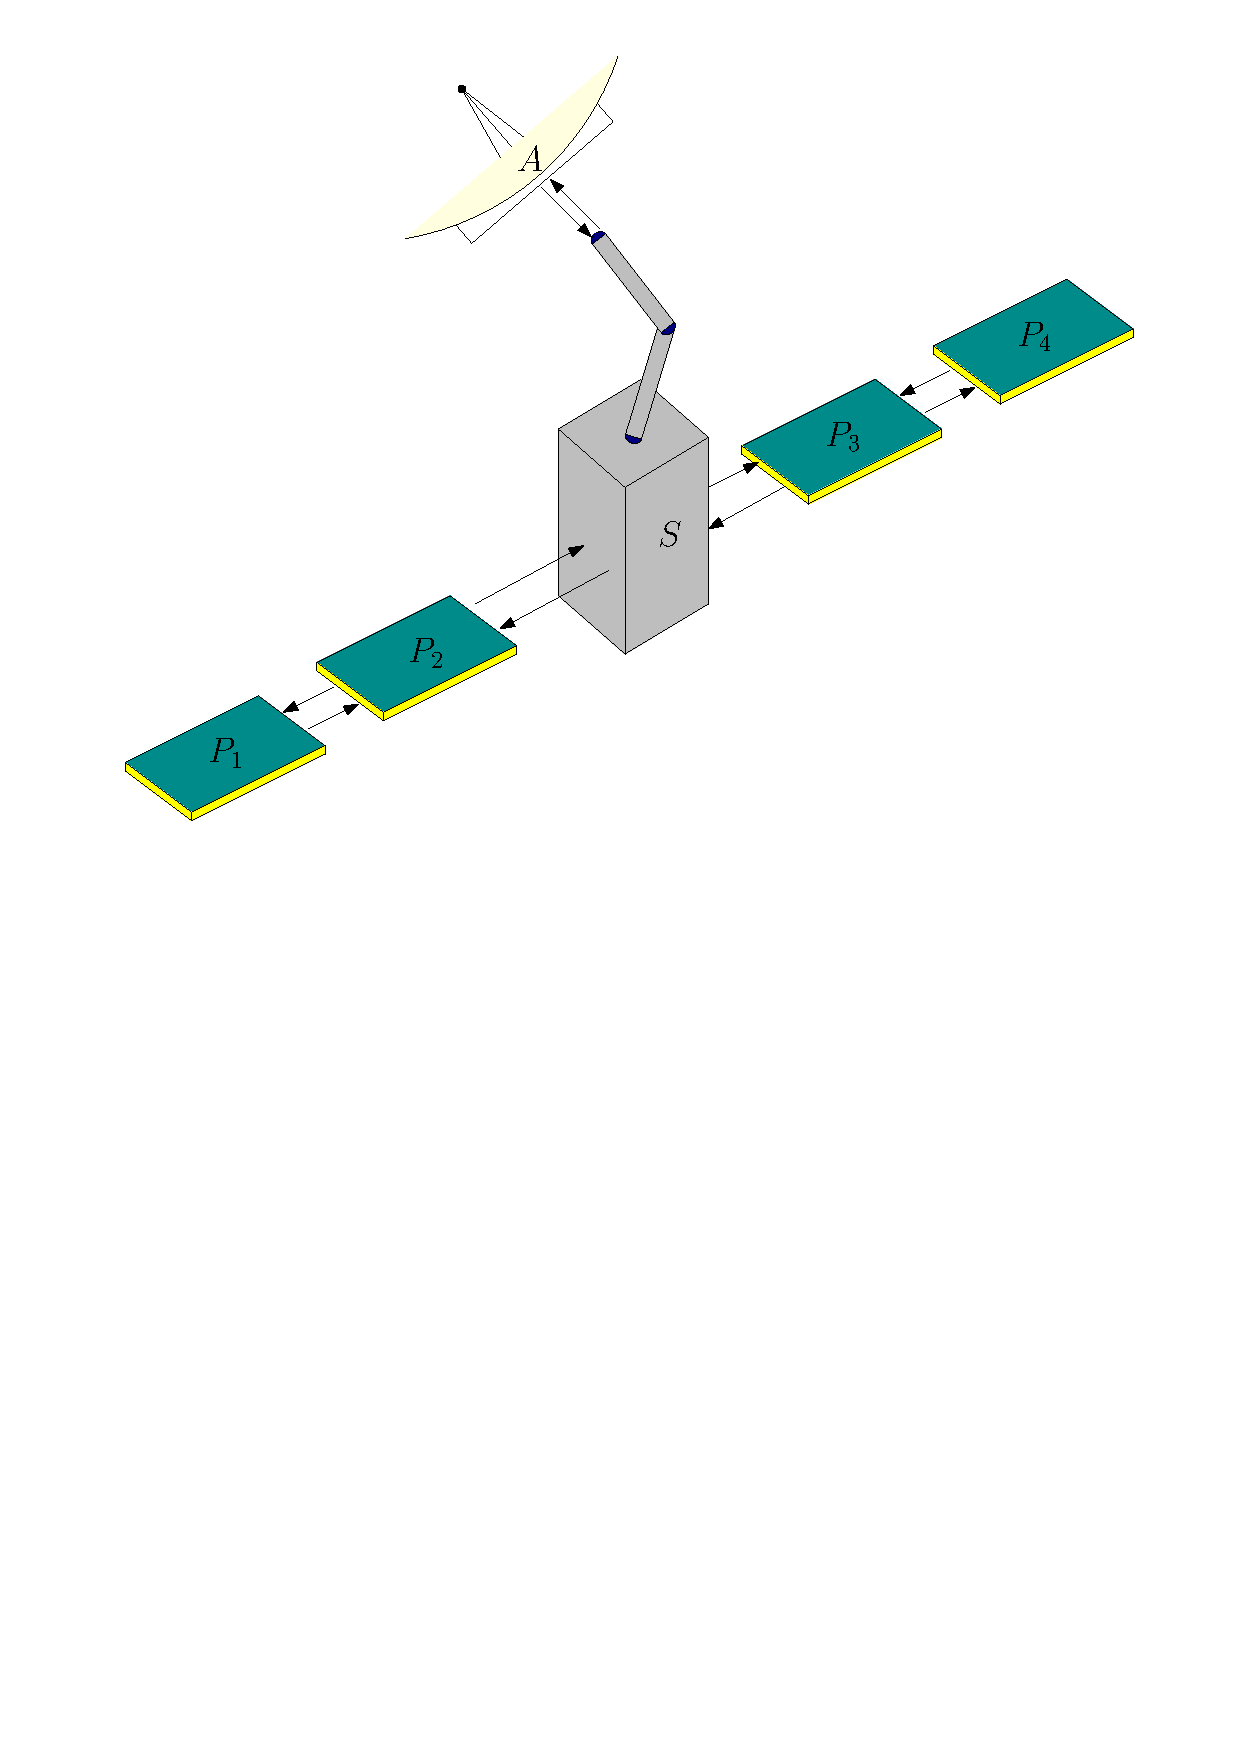
\includegraphics[width=.6\textwidth]{satellite.pdf}
		\caption{Modular scheme for a telecommunication satellite.}
		\label{fig:satellite}
	\end{figure}
	
	\paragraph{\large A unifying formalism for modeling dynamical systems}
	A very promising mathematical formalism for dealing with multiphysics problems is the port-Hamiltonian formalism, based on Hamiltonian mechanics and bond-graphs for modeling dynamical systems. At the heart of this formalism is the idea that any physical system can be described in a modular way, i.e. from its simple components, which interact with each other and with the surrounding environment through ports. The interaction port contain the information about the energy flow between the different components and between different physical domains (mechanical, electromagnetic or fluidodynamic). Modular design is fundamental in engineering, because the design of any technological system is made from simple elements that are assembled to give rise to the complexity that surrounds us. Take for example an airplane, a helicopter, a satellite (see Fig. \ref{fig:satellite}) or a cell phone: to be able to optimize their design it is essential to have a modeling tool able to decompose the complexity in a way to find the different key components. Using a unified modeling tool is an essential novelty of this project. This will allow the creation of a common infrastructure for the digital tools at the basis of digitalization, and thus facilitate its adoption in the industry.

	
	\paragraph{\large A structured methodology for the discretization of PDEs}
	The numerical algorithms used in industry are adapted to the physical nature of the problem. For mechanics, the finite element method is preferred by engineers. For fluidodynamics, finite volumes are mostly used because they guarantee the respect of conservation laws. When it is necessary to use these two approaches simultaneously, for example to treat coupled problems, their coupling poses several challenges. The two methods use different degrees of freedom (i.e. different topological entities of the mesh) and the interconnection necessarily introduces errors. A general modeling tool requires an equally general discretization method, able to guarantee the possibility of interconnecting distinct physics. This unifying formalism, the finite element exterior calculus or FEEC\footnote{Exterior calculus is a generalization of vector calculus based on differential geometry}, has been developed recently. This mathematical theory has allowed important developments for the discretization of partial differential equations from physics. It has been successfully applied to solid mechanics, fluidodynamics and electromagnetism and represents a powerful tool for multiphysics applications. 
	
	\paragraph{\large Artificial intelligence to obtain reduced models}
	Any discretization method, even the most sophisticated, leads to systems whose size easily exceeds one million unknowns. In order to optimize the design of mechanical components, these models must be simulated several times. This leads to prohibitive computational costs even for companies with the most advanced computing centers. Therefore, it is necessary to introduce reduction methods, which are supposed to build a simpler model, but still able to retain the main properties of the original system. The great majority of these methods assume that we can obtain a reduced system through an essentially linear method, i.e. the Proper Orthogonal Decomposition (POD). This assumption is not valid for any system exhibiting a nonlinear behavior and leads to overestimate the dimension of the reduced system. Thanks to the recent progress in the field of Artificial Intelligence (AI), new methods allow to obtain fast reduced models. Recently, researchers have proposed an architecture based on convolutional neural networks to obtain much faster models (by a factor of about 100) compared to high fidelity discretization. Their technique represents a non-linear extension of the commonly used methodology. The results obtained demonstrate the performance gain that can be obtained with this methodology (cf. \ref{fig:deepROM}).
	
	\begin{figure}[t]
		
		\begin{subfigure}[t]{0.465\textwidth}
			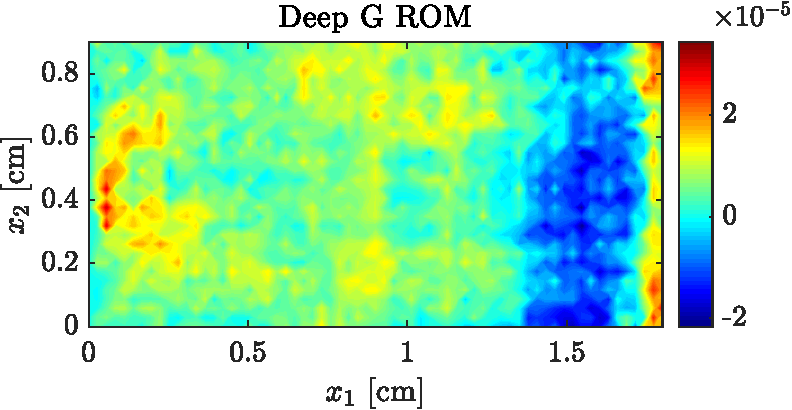
\includegraphics[width=\columnwidth]{DGROM_T_param1.pdf} 
			\caption{Reduced model obtained with a neural network}
			\label{fig:DG_ROM}
		\end{subfigure}\hfill
		\begin{subfigure}[t]{0.48\textwidth}
			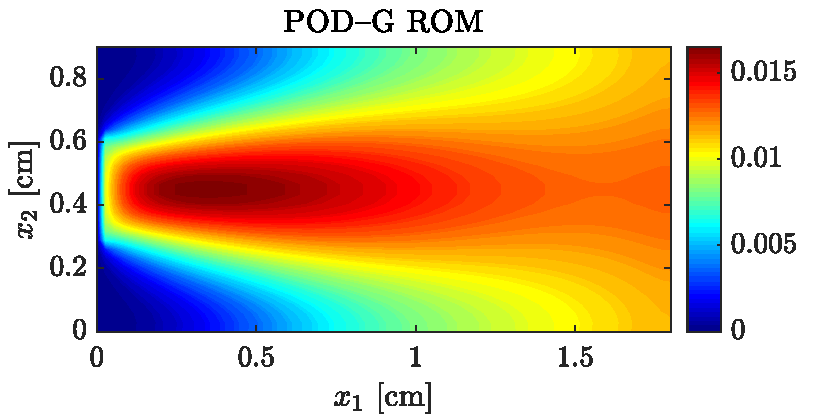
\includegraphics[width=\columnwidth]{GROM_T_param1.pdf}%
			\caption{Reduced model obtain using the linear POD.}
			\label{fig:POD_ROM}
		\end{subfigure}
		\caption[]{Error of reduced models on the temperature field for a convection-diffusion-reaction problem. By using a convolutional neural network to generate a nonlinear manifold (see Fig. \ref{fig:DG_ROM}) the error associated with the reduction is drastically reduced, from $10^{-2}$ to $10^{-5}$, compared to the POD method (see Fig. \ref{fig:POD_ROM}). Reproduced from \cite{lee2020} with permission.}%
		\label{fig:deepROM}%
	\end{figure}
	
	
	\subsection{Work Packages}
	The project is divided into three work packages:
	
	\begin{enumerate}
		\item Development of high-fidelity numerical algorithms for fluid-structure interaction problems based on the port-Hamiltonian formalism and finite elements exterior calculus.
		\item AI based reduction methods guaranteeing the respect of the physical structure. 
		\item Use of reduced models for optimization and comparison with high-fidelity models.
	\end{enumerate}
	
	Each macro-task is directly associated to a PHD thesis. For the fundamental theoretical aspects Bernhard Maschke (University of Lyon), Arjan van der Schaft (University of Groningen) and Stefano Stramigioli (University of Twente) will be the main academic interlocutors.
	
	\paragraph{\large WP1 : numerical methods for coupled fluid-structure systems\\
		Leader: Andrea Brugnoli and PhD student 1, co-supervised by Denis Matignon (DISC, ISAE)\\}
		In this first work package, we aim at obtaining coupled fluid-structure interaction models in the case where the structural part is considered deformable. Once these models are derived, the main focus of this work package will be to generate numerical algorithms for the preservation of the Hamiltonian structure. This task represents a real computational challenge, especially if we try to solve the most general possible case of fluid-structure interaction where the mechanical part is very flexible and performs rigid motions. We can then divide the task by considering problems of increasing complexity. 
		\begin{enumerate}
			\item If the structure is embedded and the deformations are small, for example an airplane wing in nominal conditions, we can use a fixed mesh over time. This is due to the fact that linear equations for elasticity can be used. 
			\item If the structure can move in a rigid manner but the deformations remain small, approaches exist to limit the complexity of the equations.
			\item In the most general case, non linear elasticity must be considered. For thin structures, intrinsic Hamiltonian formulations are already available \cite{hodges2003exact}.
		\end{enumerate}
		The PhD student will then have to design numerical methods able to adapt to this increasing complexity. The first challenge will be to solve the first case, which will not require special techniques to modify the mesh. On the contrary, the successive cases will have to use methods to consider the displacement of the elastic body (as for example the immersed boundary method). These numerical models will have to retain the physical properties of the problem (global energy conservation, tracing of energy exchanges between the different subsystems, conservation of invariants of the problem).
		
		For this first macro-task, it will be possible to extend the work done in the framework of my thesis, which gave rise to a calculation code for multiphysics application (the SCRIMP code described in \url{https://zenodo.org/record/4945329#.Yd8UJoTMJH4}). This code will be further developed to deal with fluid-structure interaction problems. The thesis co-supervisor will be Denis Matignon, because of his great expertise in numerical mathematics and port-Hamiltonian systems.
		
		For the preservation of physics within the algorithms, collaborations with Marc Gerritsma (Department of Aerodynamics at TU Delft) and Herbert Egger (Johannes Kepler University Linz) will be set up. For the fluid-structure interaction, the Office National d'Études et de Recherches Aérospatiales (ONERA), with its deep expertise in this field, will be the main contact for problems related to multiphysics coupling.
	
	\paragraph{\large WP2 : reduction of models guaranteeing the respect of the physical structure\\
		Leader: Andrea Brugnoli and PhD student 2, co-supervised by Charles Poussot-Vassal (ONERA)\\}
		
		The second challenge of the project consists in integrating techniques resulting from Artificial Intelligence
		which will be used to obtain scale models. A very promising technique in this sense is presented in \cite{lee2020}, but here the respect of physical laws is imposed a posteriori through constraints and not included at the level of the starting structure. In \cite{sun2020physics} neural networks, trained to minimize the error with respect to the mass and momentum balance, are used to get rid of the high fidelity simulation. This does not guarantee the respect of the physical structure and raises concerns about the interpretability of the results.
		
		By physical structure of the problem we mean the presence of conservation laws (associated with an anti-symmetric operator) and dissipative effects, and the variables that define the interconnection between the fluid and the solid. Keeping the physical structure of the high-fidelity simulation in the reduced representation will allow to integrate artificial intelligence tools in an interpretable way. For example, neural networks can be used to represent the energy (i.e. a function between the dimension of the state and a positive scalar), or the operator associated to the conservation of energy, or to its dissipation. 
		
		For the second macro-task, it will be possible to set up collaborations with Volker Mehrmann (TU Berlin) and George Haller (ETH Zurich).
		
	
	\paragraph{\large WP3 : optimization using reduced models\\
		Leader: Andrea Brugnoli and PhD student 3, co-supervised by Joseph Morlier (MS2M, ISAE) and Post-doc 1\\}
	
	The techniques developed in the first two work packages will allow to obtain models to describe the aeroelasticity and dynamics of robotic drones in a fluid.
	The last objective will consist in using these reduced models for optimization. This step will allow to evaluate the validity and efficiency of the reduced models compared to fine simulations. Depending on the application case, different scenarios where optimization is necessary can be evaluated (see Fig. \ref{fig:optmisation}): 
	\begin{itemize}
		\item Structural optimization of mechanical components in aeronautics, to increase aerodynamic performance (minimization of drag and thus fuel consumption, cf. Fig. \ref{fig:wing}); 
		\item Co-design of the structural part and the onboard controller. This methodology consists in optimizing the performance of the controller (which seeks, for example, to limit vibrations), at the same time as the structural characteristics of the vehicle (e.g. mass or rigidity). This type of optimization is often used for satellites (see Fig. \ref{fig:codesign_sat}).
		\item Optimal control for trajectory tracking. This type of problem frequently appears in robotics. Researchers are more and more interested in soft robotics (see Fig. \ref{fig:sofi-mit}), where the flexibility of components cannot be neglected.
	\end{itemize}
	
	Typically in industry, optimization and parametric studies are performed on surrogate models, because optimizing fine models directly leads to prohibitive computational costs. Completing these three macro-tasks will allow to better understand the trade-off between computation time and accuracy for
	applications of industrial interest. Potentially, the techniques developed in this project will provide more efficient solutions than those normally used in industry. For this task a PhD student and a PhD researcher will be hired. 
	
	\begin{figure}[t]
		\begin{subfigure}[t]{0.3\textwidth}
			\includegraphics[width=\columnwidth]{MDo_wing.png}%
			\caption{Multidisciplinary optimization of a wing: red optimized design (reproduced with permission from \cite{masColomer2021mdo}).}
			\label{fig:wing}
		\end{subfigure}\hfill
		\begin{subfigure}[t]{0.3\textwidth}
			\includegraphics[width=\columnwidth]{Codesign_satellite.pdf} 
			\caption{Model of a satellite for control/structure co-design (reproduced with permission from \cite{finozzi2022sub})}
			\label{fig:codesign_sat}
		\end{subfigure}\hfill
		\begin{subfigure}[t]{0.35\textwidth}
			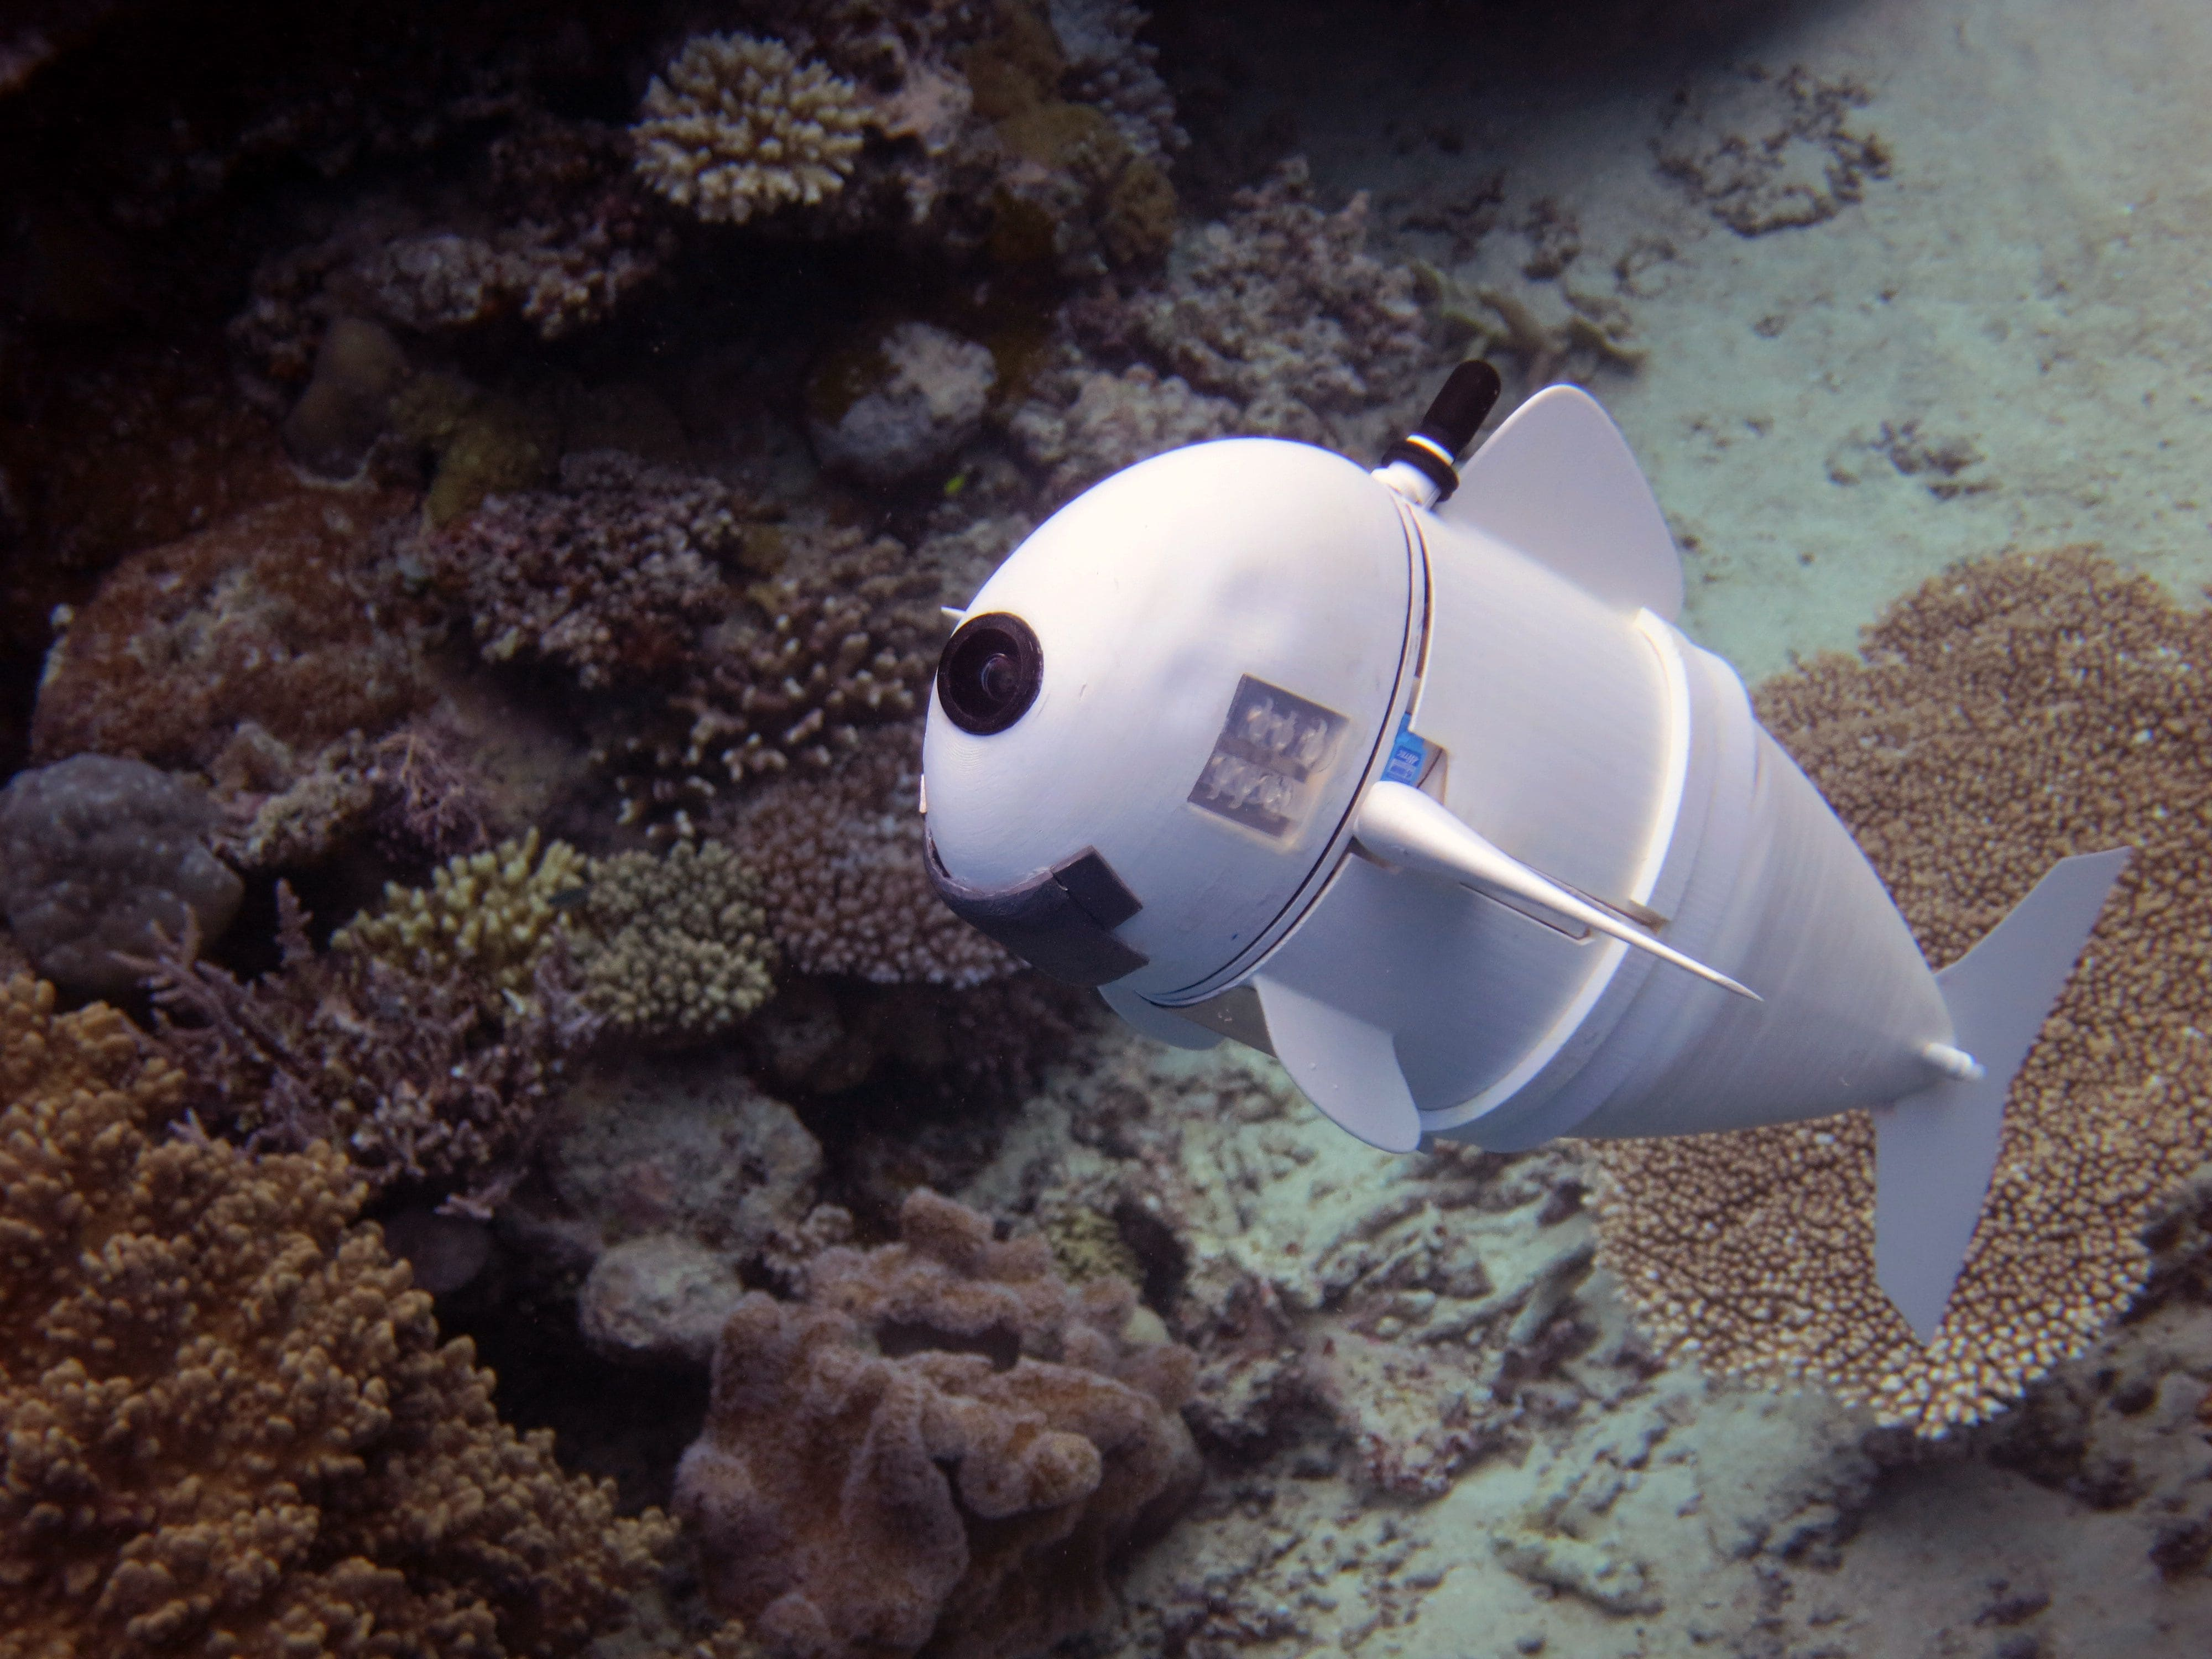
\includegraphics[width=\columnwidth]{Sofi_MIT.jpeg}%
			\caption{The MIT Sofi robotic drone (\href{https://www.csail.mit.edu/research/sofi-soft-robotic-fish}{Link to webpage})}
			\label{fig:sofi-mit}
		\end{subfigure}
		\caption[]{Application cases for optimization problems in WP3.}%
		\label{fig:optmisation}%
	\end{figure}


\bibliographystyle{unsrt}
\bibliography{biblio_dossierLL}


\end{document}
